\documentclass{article}
\usepackage[utf8]{inputenc}
\usepackage{geometry}
\usepackage{fancyhdr}
\usepackage{graphicx}
\usepackage{minted}
\usepackage{hyperref}
\usepackage{fontspec}

% document settings start
\geometry{a4paper, margin=0.9in}
\graphicspath{{./outputs/}}
\usemintedstyle{bw}
\pagestyle{fancy}
\fancyhf{}
\lhead{Numerical Methods}
\rhead{Asim Bera}
\lfoot{\href{https://github.com/asimbera/ccp-assignments.git}{https://github.com/asimbera/ccp-assignments.git}}
\rfoot{Page \thepage}

\hypersetup{
colorlinks=true,
linkcolor=blue,
filecolor=magenta,
urlcolor=blue,
}
\urlstyle{same}

\setmainfont{Overpass}
\setmonofont{Cascadia Code}

\newcommand{\problem}[2]{
  \subsection{#2}
  \underline{\emph{\Large Source Code :}}
  \inputminted[breaklines,tabsize=2]{c}{#1.c}
  \bigbreak
  \noindent
  \underline{\emph{\Large Program Output :}}
  \bigbreak
  \noindent
  \includegraphics[width=110mm,scale=0.5]{#1}
  % \newpage
  % \bigbreak
  \vspace{1cm}
}

% document settings end

\begin{document}
\begin{titlepage}
  \begin{center}
    \vspace*{2cm}
    
\includegraphics[width=0.3\textwidth]{logo}\\
    \vspace{0.5cm}
    {\huge CENTRAL CALCUTTA POLYTECHNIC}\\
    \vspace{0.4cm}
    21, Convent Road, Philips, Sealdah, Kolkata, West Bengal 700014\\
    \vspace{0.8cm}
    {\Large \textsc{Dept. : Computer Science and Technology}}
  \end{center}
  \vspace{1.2cm}
  \textsc{
    \huge
    \begin{itemize}
      \item Name : Asim Bera
      \item Roll : DCCPCSTS6
      \item Number : 10005504
      \item Reg number : D192005209
      \item Subject : Advanced Java Programming
      \item Session : 2021-2022
    \end{itemize}
  }

\end{titlepage}

\newpage
\pagenumbering{roman}
\tableofcontents
\newpage
\pagenumbering{arabic}
\setcounter{page}{1}
\section{Numerical Methods Lab}

\subsection{Write a C Program to find out the value of f(2.35) using Newton's Forward Interpolation Formula from the following table}
\begin{center}
\begin{tabular}{c|c|c|c|c|c}
  x: & 2.00 & 2.25 & 2.50 & 2.75 & 3.00 \\
  f(x): & 9.00 & 10.06 & 11.25 & 12.56 & 14.00
\end{tabular}
\end{center}
\bigbreak
\underline{\emph{\Large Source Code :}}
\inputminted[breaklines,tabsize=2]{c}{1.c}
\bigbreak
\noindent
\underline{\emph{\Large Program Output :}}
\bigbreak
\noindent
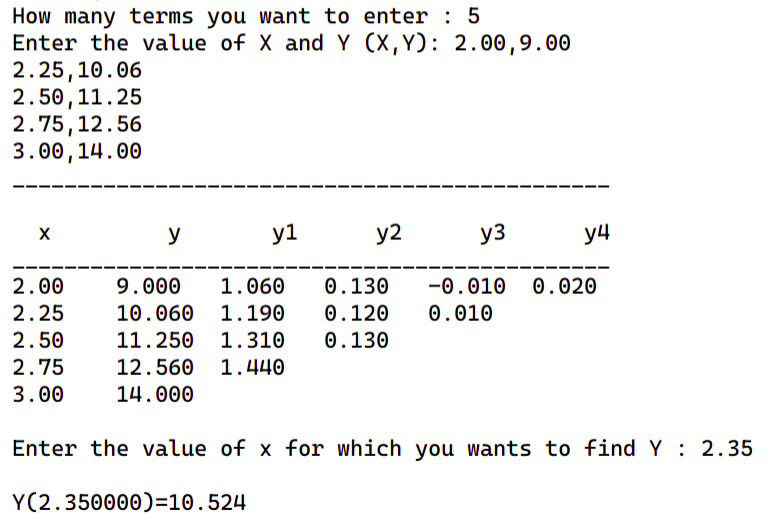
\includegraphics[width=110mm,scale=0.5]{outputs/1}

\subsection{Write a C Program to find out the value of f(4.25) using Newton's Backward Interpolation Formula from the following table}
\begin{center}
\begin{tabular}{c|c|c|c|c|c}
  x: & 2.5 & 3.0 & 3.5 & 4.0 & 4.5 \\
  f(x): & 9.75 & 12.75 & 15.70 & 19.52 & 23.75
\end{tabular}
\end{center}
\bigbreak
\underline{\emph{\Large Source Code :}}
\inputminted[breaklines,tabsize=2]{c}{2.c}
\bigbreak
\noindent
\newpage
\underline{\emph{\Large Program Output :}}
\bigbreak
\noindent
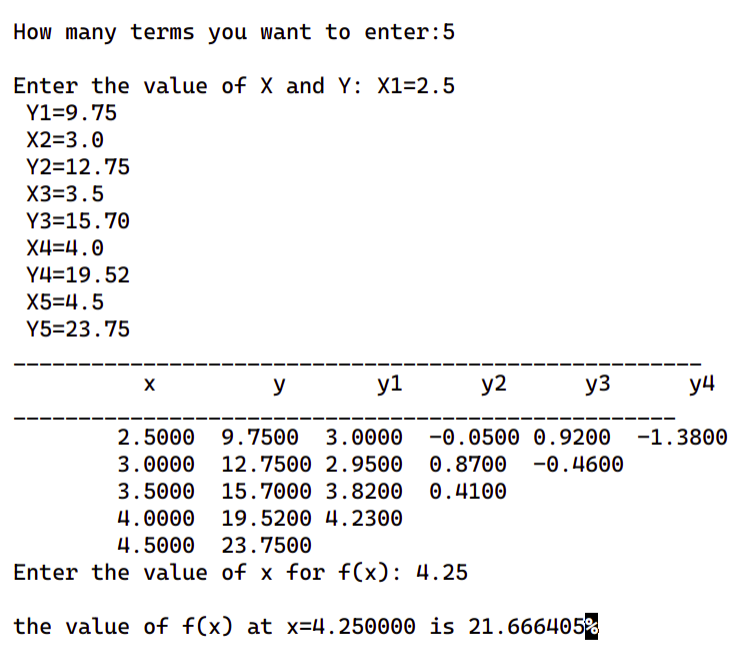
\includegraphics[width=110mm,scale=0.5]{outputs/2}

\subsection{Write a C Program to find out the value of f(4.25) using Newton's Divide Difference Interpolation Formula from the following table}
\begin{center}
\begin{tabular}{c|c|c|c|c|c}
  x: & 2.5 & 3.0 & 4.5 & 4.75 & 6.0 \\
  f(x): & 8.85 & 11.45 & 20.66 & 22.85 & 38.60
\end{tabular}
\end{center}
\bigbreak
\underline{\emph{\Large Source Code :}}
\inputminted[breaklines,tabsize=2]{c}{3.c}
\bigbreak
\noindent
\newpage
\underline{\emph{\Large Program Output :}}
\bigbreak
\noindent
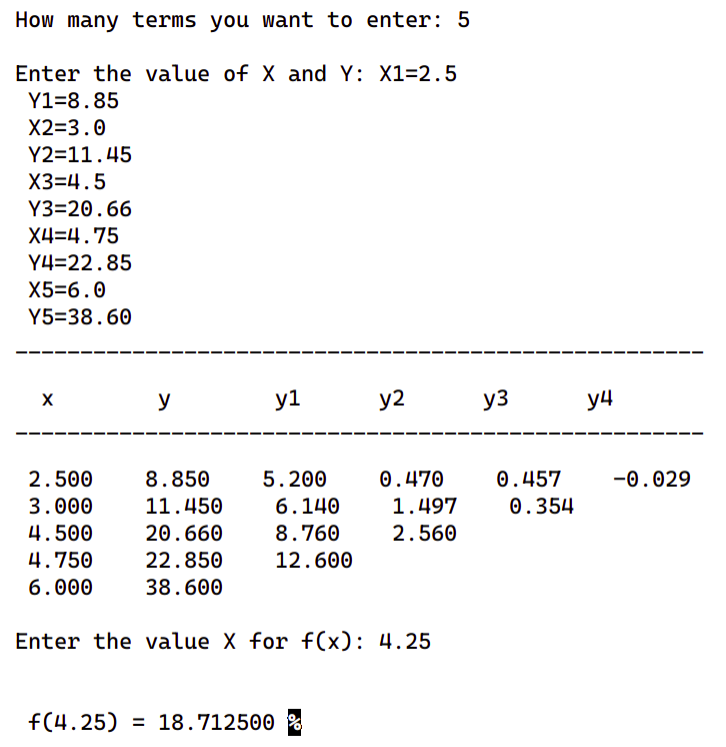
\includegraphics[width=110mm,scale=0.5]{outputs/3}

\problem{4}{Write a C Program to evaluate $\int_{2}^{1} \frac{1}{1+x^2} \,dx$ using Trapezoidal rule with 6 intervals.}
\problem{5}{Write a C Program to evaluate $\int_{2}^{1} \frac{x}{1+x} \,dx$ using Simpson's 1/3rd Rule with 6 intervals.}
\problem{6}{Write a C Program to find the root of the equation $x^3 + x^2 + x + 7 = 0$ using Bisection Method.}
\problem{7}{Write a C Program to find the root of the equation $x^3 - x -3 = 0$ using Newton Raphson Mehtod.}

\end{document}
